\section{Metodologia}

\subsection{Conjunto de dados}

O estudo utiliza implementações de código geradas por cinco modelos de linguagem de grande porte (LLMs) para tarefas de programação provenientes de três conjuntos: \textbf{CEJava}, \textbf{CEPython} e \textbf{HumanEval}.

Os conjuntos CEJava e CEPython derivam do \textit{CoderEval}, um benchmark de geração de código ``pragmática'' composto por funções extraídas de projetos reais que dependem do contexto do repositório. O CEJava reúne 230 tarefas em Java e o CEPython, 230 tarefas em Python; este último foi complementado com contextos recuperados por RAG. O HumanEval é um conjunto de 164 tarefas de programação em Python, em geral autocontidas (função com assinatura e testes), originalmente proposto por Chen et al. (2021).

Os cinco modelos geradores foram: DeepSeek-Coder-1.3B, DeepSeek-Coder-7B, CodeLlama-7B, GPT-4 e DeepSeek-R1. Para cada tarefa, cada modelo gerou uma implementação, resultando em cinco implementações por tarefa e em 3.120 implementações no total (Tabela~\ref{tab:datasets}).

\begin{table}[ht]
    \centering
    \caption{Composição do conjunto de dados por origem.}
    \label{tab:datasets}
    \begin{tabular}{llrrr}
        \hline
        \textbf{Conjunto} & \textbf{Linguagem} & \textbf{Tarefas} & \textbf{Implementações} & \textbf{Anotadas} \\
        \hline
        CEJava    & Java   & 230 & 1.150 & 547 \\
        CEPython  & Python & 230 & 1.150 & 426 \\
        HumanEval & Python & 164 &   820 & 161 \\
        \hline
        \textbf{Total} & & \textbf{624} & \textbf{3.120} & \textbf{1.134} \\
        \hline
    \end{tabular}
\end{table}

Cada implementação foi avaliada quanto à presença de alucinações segundo a taxonomia proposta por Liu et al., que define 12 tipos distintos. Essa anotação manual está disponível para 1.134 das 3.120 implementações (36,3\%); as demais 1.986 não possuem rótulo. Como a ausência de rótulo não equivale à ausência de alucinação, essas implementações não são tratadas como tal e são excluídas da análise de associação.

Além disso, todas as 3.120 implementações foram analisadas individualmente pelo SonarQube, uma ferramenta de análise estática que verifica a conformidade do código com regras de qualidade e registra uma \textit{issue} a cada regra violada. O scan foi executado com o SonarQube 10.0.0, com os perfis padrão (\textit{Sonar way}) para Java e Python. O scan completo identificou 71 regras distintas considerando o identificador completo da regra, que inclui a linguagem à qual pertence, como, por exemplo, \texttt{java:S1854} e \texttt{python:S1854}, totalizando 1.426 issues. Regras Java e Python com o mesmo identificador numérico foram mantidas separadas, uma vez que pertencem a analisadores específicos de cada linguagem e não se assumiu equivalência entre elas.

Como a análise de associação depende da anotação manual de alucinação, ela é restrita ao subconjunto anotado. A forma de seleção dos pares alucinação--regra efetivamente analisados é descrita na Subseção~\ref{sec:elegibilidade}.

\subsection{Preparação dos dados}

\subsubsection{Binarização das variáveis}

Para permitir a análise da relação entre os tipos de alucinação e as regras do SonarQube, ambas as variáveis foram representadas por indicadores binários.

Para cada tipo de alucinação $X$, definiu-se:

\[
X =
\begin{cases}
1, & \text{se a implementação apresenta a alucinação;}\\
0, & \text{caso contrário.}
\end{cases}
\]

Analogamente, para cada regra do SonarQube $Y$:

\[
Y =
\begin{cases}
1, & \text{se a implementação apresenta uma violação da regra;}\\
0, & \text{caso contrário.}
\end{cases}
\]

Dessa forma, foi construída uma matriz no nível da implementação, com uma linha para cada implementação do conjunto anotado e indicadores binários para os 12 tipos de alucinação e para as 60 regras do SonarQube presentes nesse conjunto.

\subsubsection{Elegibilidade das implementações e seleção dos pares avaliáveis}\label{sec:elegibilidade}

O objetivo é investigar, para cada par formado por um tipo de alucinação $X$ e uma regra do SonarQube $Y$, se a regra $Y$ é proporcionalmente mais frequente entre as implementações que apresentam a alucinação $X$. Para que um par possa ser analisado, duas condições precisam ser satisfeitas.

Primeiro, é necessário que exista anotação manual de alucinação, pois $X$ só está definido nas 1.134 implementações anotadas; por isso a análise é restrita a esse subconjunto.

Segundo, é necessário que a implementação pertença à linguagem da regra. Como cada regra é definida pelo analisador de uma linguagem, regras com prefixo \texttt{java:} só podem ser violadas por código Java e são avaliadas apenas nas implementações de CEJava; regras com prefixo \texttt{python:} só podem ser violadas por código Python e são avaliadas nas implementações de CEPython e HumanEval. Essa restrição evita tratar a ausência de uma violação Java em um código Python como se fosse uma observação de valor $Y=0$. O subconjunto de implementações anotadas da linguagem correspondente é denominado, neste estudo, \textit{conjunto de implementações elegíveis} para a regra.

A partir dessas duas condições, a seleção dos pares analisados segue quatro passos:

\begin{enumerate}
    \item \textbf{Regras disponíveis.} Das 71 regras identificadas no scan completo, apenas 60 ocorrem entre as implementações anotadas (32 Java e 28 Python); as demais não podem ser relacionadas a nenhum tipo de alucinação anotado.
    \item \textbf{Pares candidatos.} Combinando os 12 tipos de alucinação com as 60 regras, obtêm-se $12 \times 60 = 720$ pares candidatos.
    \item \textbf{Avaliabilidade.} Um par é descartado quando o tipo $X$ não ocorre em nenhuma implementação elegível para a regra $Y$, pois não haveria grupo com $X$ para comparar com o grupo sem $X$. Isso elimina 124 pares com $X$ ausente (9 dos 12 tipos ocorrem em implementações elegíveis a regras Java e 11 dos 12 em Python).
    \item \textbf{Pares avaliáveis.} Restam \textbf{596 pares avaliáveis}: 288 com regras Java e 308 com regras Python. As análises a seguir referem-se a esses pares.
\end{enumerate}

A caracterização de esparsidade (Subseção~\ref{sec:esparcidade}) não exclui pares, mas registra quanta informação cada um sustenta.

\subsubsection{Níveis de análise}

A análise foi estruturada em dois níveis: implementação e tarefa.

No nível da implementação, cada uma das 1.134 implementações com anotação manual ocupa uma linha da matriz de dados e é analisada separadamente. A presença da alucinação $X$ e da regra $Y$ refere-se, portanto, à mesma implementação.

No nível da tarefa, as implementações anotadas correspondentes à mesma
tarefa são agregadas em uma única unidade de análise. Para cada tipo
de alucinação e regra do SonarQube, uma tarefa recebe valor 1 quando
pelo menos uma de suas implementações anotadas apresenta a característica
analisada, e valor 0 quando nenhuma implementação anotada a apresenta.

Consequentemente, a presença simultânea de uma alucinação $X$ e de uma
regra $Y$ no nível da tarefa não implica que ambas tenham ocorrido na
mesma implementação. Ela indica que, entre as implementações associadas
àquela tarefa, pelo menos uma apresentou $X$ e pelo menos uma apresentou
$Y$.

\subsection{Procedimento de análise exploratória}

Este estudo caracteriza-se como um \textbf{estudo de caso exploratório}. Seu objetivo é descrever os padrões observados e gerar hipóteses sobre a relação entre tipos de alucinação e regras do SonarQube, e não confirmar associações na população. Por isso, as medidas descritas a seguir são interpretadas como descritivas e nenhuma conclusão causal lhes é atribuída.

Para caracterizar a frequência marginal das variáveis, considerou-se
$n_X$ o número de implementações elegíveis que apresentam
a alucinação $X$, e $n_Y$ o número de
implementações elegíveis que apresentam a violação $Y$.
A Tabela~\ref{tab:distribuicao_frequencias_marginais} apresenta a
distribuição dessas frequências entre os 596 pares avaliáveis, no nível da implementação. 

\begin{table}[ht]
    \centering
    \caption{Distribuição das frequências marginais ($n_X$ e $n_Y$) nos 596 pares
    alucinação--regra avaliáveis, no nível da implementação. Ambas as
    frequências são contadas dentro do conjunto elegível de cada regra.}
    \label{tab:distribuicao_frequencias_marginais}
    
    \begin{tabular}{lrr}
        \hline
        \textbf{Estatística} 
        & $\boldsymbol{n_X}$ 
        & $\boldsymbol{n_Y}$ \\
        \hline
        
        Média              & 59,65  & 6,96 \\
        1º quartil (25\%)  & 3      & 1    \\
        Mediana (50\%)     & 26     & 1    \\
        3º quartil (75\%)  & 129    & 4    \\
        90º percentil      & 167,5  & 11   \\
        95º percentil      & 172    & 14   \\
        Máximo             & 291    & 197  \\
        
        \hline
    \end{tabular}
\end{table}

Observa-se que as violações do SonarQube apresentam frequências
particularmente baixas. A mediana de $n_Y$ foi igual a 1, indicando
que, em metade dos pares avaliáveis, a respectiva regra do SonarQube
foi observada em no máximo uma implementação elegível. O primeiro
quartil de $n_Y$ também foi igual a 1, e o maior valor observado foi
197, mostrando a elevada concentração de regras com baixa frequência de
ocorrência e a forte assimetria da distribuição.

Como pode ser observado na Tabela~\ref{tab:distribuicao_frequencias_marginais}, há elevada esparsidade observada nas combinações entre tipos de alucinação e regras do SonarQube e, devido a esta característica, a análise concentra-se na caracterização dos padrões observados nos dados, sem utilizar testes de significância como critério para determinar a existência de associações.

Essa escolha descritiva tem uma consequência que deve ser explicitada: ao examinar 596 pares sem qualquer ajuste para comparações múltiplas, valores extremos de $\Delta$ ou de \textit{odds ratio} são esperados apenas por variação amostral. Por isso, nenhum par é destacado com base exclusivamente na magnitude dessas medidas, e cada padrão reportado é acompanhado da sua tabela de contingência completa ($a$, $b$, $c$, $d$) e das frequências que o sustentam.

A análise considera conjuntamente a ocorrência das variáveis, a direção e a magnitude das diferenças observadas e a quantidade de observações que sustentam cada padrão.

\subsubsection{Construção das tabelas de contingência}

Para cada par formado por um tipo de alucinação $X$ e uma regra do
SonarQube $Y$, foi construída uma tabela de contingência $2\times2$,
conforme apresentado na Tabela~\ref{tab:contingencia}.

\begin{table}[ht]
    \centering
    \caption{Estrutura da tabela de contingência para cada par
    alucinação--regra.}
    \label{tab:contingencia}
    \begin{tabular}{lcc}
        \hline
        & $Y=1$ & $Y=0$ \\ 
        \hline
        $X=1$ 
        & $a$: $X$ e $Y$ presentes
        & $b$: apenas $X$ presente \\

        $X=0$
        & $c$: apenas $Y$ presente
        & $d$: $X$ e $Y$ ausentes \\
        \hline
    \end{tabular}
\end{table}

A partir das células da tabela de contingência, foram calculadas as
frequências marginais:

\[
n_{X=1}=a+b,
\qquad
n_{X=0}=c+d,
\]

\[
n_{Y=1}=a+c,
\qquad
n_{Y=0}=b+d.
\]

Essas frequências são utilizadas tanto para caracterizar a ocorrência
das variáveis quanto para contextualizar as medidas exploratórias
calculadas posteriormente.

\subsubsection{Caracterização da esparsidade}\label{sec:esparcidade}

Antes da interpretação das medidas de associação, foi avaliada a
esparsidade das tabelas de contingência.

Foram examinadas as frequências marginais de $X$ e $Y$, o número de
ocorrências conjuntas e a presença de células com frequência zero.

Não foi adotado um número mínimo de coocorrências como critério
automático de exclusão. A ausência de coocorrência não implica
necessariamente ausência de um padrão de associação, pois $X$ e $Y$
podem ocorrer individualmente com frequência e, ainda assim, não
ocorrer conjuntamente.

Os pares foram, portanto, classificados estruturalmente nas seguintes
categorias:

\begin{description}

    \item[$X$ ausente:]
    não existem implementações com $X$ no conjunto elegível para a
    regra $Y$, impossibilitando a comparação entre implementações com
    e sem $X$;

    \item[Sem coocorrência:]
    $X$ e $Y$ ocorrem no conjunto elegível, mas nenhuma implementação
    apresenta ambos simultaneamente;

    \item[Coocorrência completa:]
    existe pelo menos uma ocorrência conjunta de $X$ e $Y$, e todas
    as quatro células da tabela de contingência possuem frequência
    diferente de zero;

    \item[Coocorrência com célula zero:]
    existe pelo menos uma ocorrência conjunta de $X$ e $Y$, mas uma
    das células comparativas da tabela apresenta frequência zero.

\end{description}

Essa classificação permite distinguir a ausência de informação para
comparação da ausência efetivamente observada de coocorrência.

\subsubsection{Diferença de proporções}

Para cada par avaliável, foi calculada a proporção de implementações com a violação $Y$ entre aquelas que apresentaram a alucinação $X$:

\[
P(Y=1\mid X=1)
=
\frac{a}{a+b},
\]

e a proporção correspondente entre implementações sem a alucinação:

\[
P(Y=1\mid X=0)
=
\frac{c}{c+d}.
\]

A diferença entre essas proporções foi definida como:

\[
\Delta =
P(Y=1\mid X=1)
-
P(Y=1\mid X=0).
\]

Valores positivos de $\Delta$ indicam que, no conjunto observado, a regra $Y$ é proporcionalmente mais frequente entre implementações com a alucinação $X$. Valores negativos indicam que $Y$ é proporcionalmente mais frequente entre implementações sem $X$. Valores próximos de zero indicam proporções semelhantes entre os dois grupos.

A diferença de proporções é utilizada como medida descritiva da direção e da magnitude do padrão observado, e não como evidência inferencial de associação na população.

\subsubsection{Odds ratio}

Como medida complementar de associação, foi considerado o \textit{odds ratio} (OR):

\[
OR=\frac{ad}{bc}.
\]

Quando todas as células possuem frequência diferente de zero, valores de $OR>1$ indicam maior \textit{odds} de ocorrência de $Y$ entre implementações com $X$, enquanto valores de $OR<1$ indicam menor \textit{odds}. Um valor de $OR=1$ corresponde à igualdade das \textit{odds} entre os grupos.

Entretanto, devido à ocorrência frequente de células com valor zero, o OR bruto não é utilizado isoladamente para ordenar ou classificar os pares. Valores iguais a zero ou que tendem ao infinito são interpretados conjuntamente com a configuração da tabela de contingência e com as frequências que lhes deram origem.

Em particular, uma medida de associação extrema baseada em poucas observações não é interpretada da mesma maneira que uma medida de magnitude semelhante sustentada por um número maior de ocorrências.

\subsubsection{Suporte observacional}

A magnitude das diferenças observadas é analisada conjuntamente com o suporte observacional de cada par.

Para isso, são consideradas principalmente as frequências:

\[
n_X=n_{X=1}=a+b
\]

e

\[
n_Y=n_{Y=1}=a+c.
\]

Essa avaliação é necessária porque diferenças de proporções elevadas podem ser produzidas por um número muito pequeno de observações. Por exemplo, uma proporção de 100\% pode corresponder tanto a uma ocorrência em uma única observação quanto a um padrão repetido em um número elevado de implementações.

Como diagnóstico exploratório adicional, considera-se o suporte mínimo:

\[
S=\min(n_X,n_Y).
\]

Essa quantidade representa a menor frequência marginal entre a alucinação e a regra analisadas. O suporte mínimo não constitui uma medida de associação nem um critério estatístico de significância. Ele é utilizado apenas para auxiliar a interpretação da magnitude dos padrões observados.

A relação entre $\Delta$ e as frequências $n_X$, $n_Y$ e $S$ é examinada graficamente para verificar se diferenças extremas estão concentradas principalmente em pares com baixo suporte observacional.

Não são excluídos pares com base em um ponto de corte. Para fins de destaque e interpretação, entretanto, considera-se que um par tem \textit{suporte observacional suficiente} quando $S \ge 10$ e quando ao menos cinco implementações apresentam a ocorrência conjunta ($a \ge 5$); pares abaixo desse limiar permanecem descritos, mas não são destacados como padrões. Magnitude, direção e suporte observacional são considerados conjuntamente na interpretação dos padrões.

\subsubsection{Controle por correção funcional}

Como a anotação manual concentra-se em código que não passou nos testes, a correção funcional pode confundir a relação entre alucinação e regra: código incorreto tende a acumular tanto alucinações quanto violações do SonarQube. Para separar esse efeito, além da análise sobre o conjunto de pares avaliáveis, as medidas são recalculadas dentro de estratos definidos pelo resultado da execução (\textit{evaluation result}): implementações que passam e implementações que falham nos testes. Um padrão que se mantém nos dois estratos é menos compatível com um efeito meramente decorrente da correção funcional do que um padrão observado apenas no conjunto agregado. Os resultados são reportados de forma estratificada para os pares com suporte observacional suficiente.

\subsubsection{Identificação dos padrões exploratórios}

A caracterização de cada par alucinação--regra considera conjuntamente:

\[
a,\quad
n_X,\quad
n_Y,\quad
P(Y\mid X),\quad
P(Y\mid \neg X),\quad
\Delta
\]

e, quando informativo, o \textit{odds ratio}.

A análise busca identificar:

\begin{itemize}
    \item padrões positivos, nos quais a ocorrência de $Y$ é proporcionalmente maior entre implementações com $X$;
    \item padrões negativos, nos quais a ocorrência de $Y$ é proporcionalmente menor entre implementações com $X$;
    \item casos de ausência de coocorrência em que $X$ e $Y$ apresentam frequências marginais suficientes para que esse padrão seja descritivamente relevante;
    \item valores extremos associados a frequências muito baixas, que devem ser interpretados com cautela.
\end{itemize}

Dessa forma, nenhum par é caracterizado como relevante exclusivamente com base em um valor elevado de $\Delta$ ou do OR. A interpretação considera simultaneamente a direção, a magnitude e o suporte observacional do padrão.

\subsection{Análise no nível da tarefa}

No nível da tarefa, a unidade de análise deixa de ser a implementação individual e passa a ser a tarefa de programação. Como cada tarefa possui cinco implementações geradas por modelos distintos, essa agregação permite investigar se uma tarefa que manifesta um tipo de alucinação também tende a manifestar a violação de uma regra do SonarQube, independentemente do modelo que a produziu.

A anotação manual de alucinação cobre 1.134 implementações, distribuídas em 433 tarefas, com uma a cinco implementações anotadas por tarefa (média de 2,62). O conjunto de análise no nível da tarefa é, portanto, formado por essas 433 tarefas, e a agregação considera apenas as implementações anotadas de cada tarefa.

Para cada alucinação $X$:

\[
X_{\text{task}}=
\begin{cases}
1, & \text{se pelo menos uma implementação anotada da tarefa apresenta }X;\\
0, & \text{caso contrário.}
\end{cases}
\]

Analogamente, para cada regra $Y$:

\[
Y_{\text{task}}=
\begin{cases}
1, & \text{se pelo menos uma implementação anotada da tarefa apresenta }Y;\\
0, & \text{caso contrário.}
\end{cases}
\]

A agregação é feita pelo critério \textit{any}. Por consequência, a ocorrência conjunta de $X$ e $Y$ no nível da tarefa não implica que ambas tenham ocorrido na mesma implementação: ela indica que, entre as implementações anotadas da tarefa, pelo menos uma apresentou $X$ e pelo menos uma apresentou $Y$. Em relação ao nível da implementação, essa agregação reduz a esparsidade e amplia a sensibilidade da análise, ao custo de eliminar o pareamento entre alucinação e regra dentro de uma mesma implementação.

A análise exploratória no nível da tarefa segue a mesma lógica geral do nível da implementação: construção das tabelas de contingência $2\times2$ para os mesmos 596 pares avaliáveis (12 tipos de alucinação e as 60 regras presentes no conjunto anotado), cálculo das frequências marginais $n_X$ e $n_Y$, diferença de proporções $\Delta$, \textit{odds ratio} (interpretado com cautela) e suporte observacional $S=\min(n_X,n_Y)$. A classificação estrutural de esparsidade é reaplicada, esperando-se, neste nível, uma densidade maior do que a observada no nível da implementação.

As visualizações são as mesmas adotadas no nível da implementação, em particular a relação entre $\Delta$ e o suporte observacional $S$, o que permite comparar os padrões identificados nos dois níveis de análise.

\subsection{Escopo e limitações da análise}

A análise de associação é conduzida sobre o subconjunto de 1.134 implementações com anotação manual, o que restringe o alcance das conclusões. Essa anotação não é distribuída de forma uniforme: a cobertura é de 47,6\% em CEJava, 37,0\% em CEPython e 19,6\% em HumanEval, e de 42,7\% entre as implementações que falham nos testes contra 10,5\% entre as que passam. O conjunto analisado é, portanto, composto majoritariamente por código que não passou nos testes e sobre-representa determinados conjuntos e modelos. Por isso, as conclusões valem para esse subconjunto anotado e não devem ser generalizadas para todo o código gerado por LLMs.

Além disso, as observações não são independentes: cada tarefa possui até cinco implementações, geradas por modelos distintos, e o modelo pode influenciar tanto a presença de alucinações quanto a de violações. Como consequência, a análise é descritiva e não emprega testes de significância, de modo que as frequências e medidas reportadas não devem ser interpretadas como evidência inferencial sobre a população.

\subsection{Resultados preliminares}

A pré-análise descritiva foi conduzida sobre os 596 pares avaliáveis, nos níveis da implementação e da tarefa. A Tabela~\ref{tab:padroes_impl} lista os pares com suporte observacional suficiente ($S \ge 10$ e $a \ge 5$), ordenados por $|\Delta|$; a Figura~\ref{fig:delta_suporte} relaciona $\Delta$ ao suporte observacional; e a Tabela~\ref{tab:padroes_task} apresenta o nível da tarefa.

Dois resultados se destacam. Primeiro, a maioria dos pares é vazia: no nível da implementação, 472 dos 596 pares (79,2\%) não apresentam nenhuma coocorrência entre $X$ e $Y$; no nível da tarefa, 407 (68,3\%), ainda majoritário. Segundo, mesmo entre os pares com suporte suficiente as diferenças são pequenas: no nível da implementação, $|\Delta|$ não passa de 0,08 e a maior parte envolve a regra genérica \texttt{java:S1854}, que concentra 215 das coocorrências, contra 36 da segunda regra (\texttt{python:S1172}).

A contribuição por modelo revela confundimento: vários padrões se concentram em um único LLM --- 8 dos 9 casos de \textit{Library/Project} $\times$ \texttt{python:S3776} e 11 dos 15 de \textit{Library/Project} $\times$ \texttt{java:S1144} vêm do DeepSeek-R1. Além disso, a estratificação por correção funcional não confirma os padrões: no estrato de implementações que passam nos testes (65 implementações), o principal destaque do nível da implementação não reaparece e as associações com \texttt{java:S1854} chegam a inverter de sinal.

Em conjunto, os resultados sugerem que regras do SonarQube não funcionam como \textit{proxy} geral de tipos específicos de alucinação e que as poucas associações observadas são fracas e confundidas. Esses padrões são discutidos na seção de discussão.

\begin{figure}[ht]
    \centering
    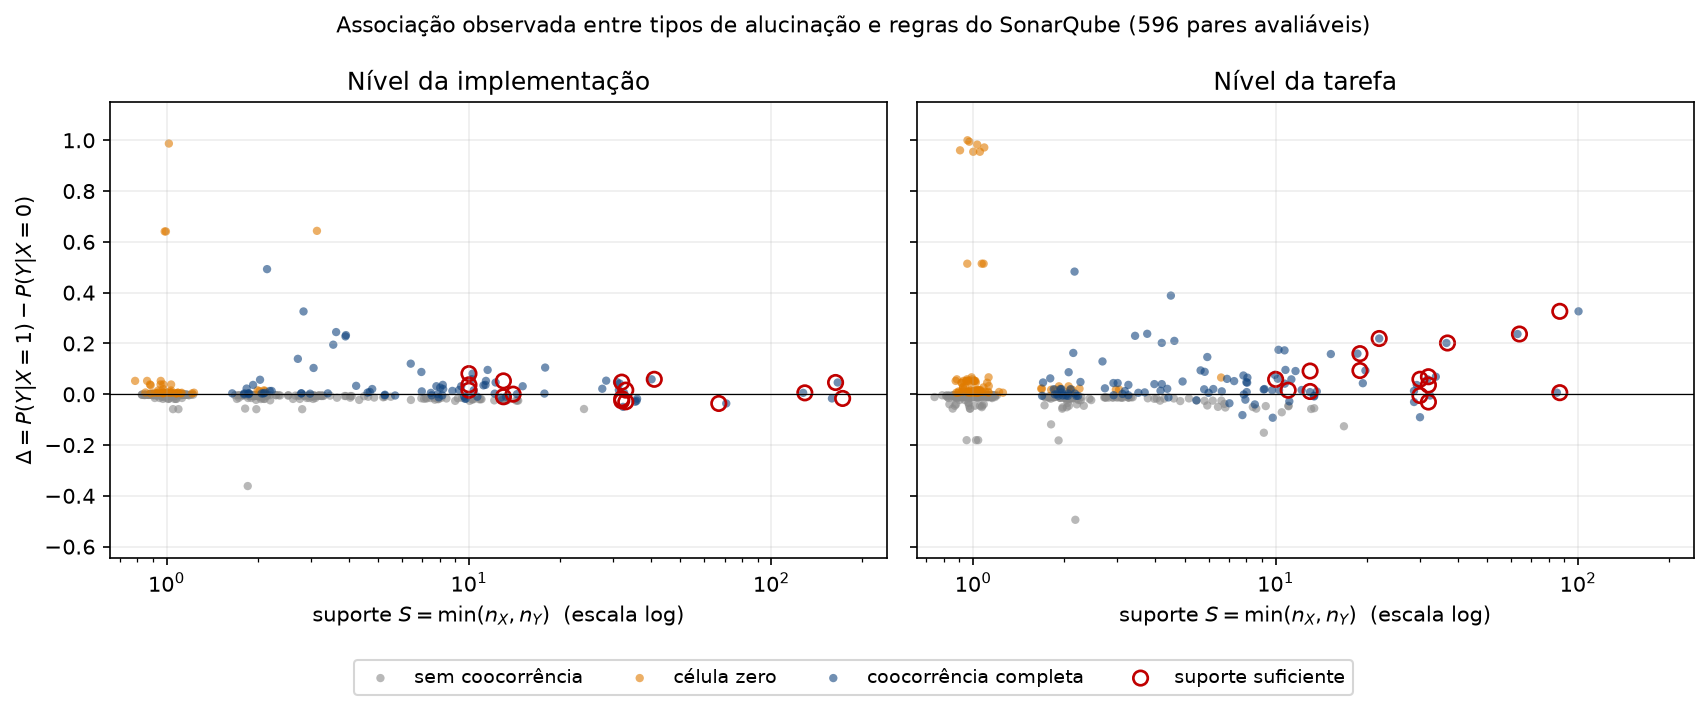
\includegraphics[width=\textwidth]{fig-delta-suporte.png}
    \caption{Relação entre $\Delta$ e o suporte observacional $S=\min(n_X,n_Y)$ (escala logarítmica), por classe de esparsidade, nos níveis da implementação (esquerda) e da tarefa (direita). Círculos vazados indicam suporte suficiente ($S \ge 10$ e $a \ge 5$).}
    \label{fig:delta_suporte}
\end{figure}

\begin{table}[ht]
\centering
\caption{Pares alucinação--regra com suporte suficiente ($S\ge 10$ e $a\ge 5$), por $|\Delta|$ --- nível da implementação.}
\label{tab:padroes_impl}
\begin{tabular}{llrrrr}
\hline
Alucinação ($X$) & Regra ($Y$) & $a$ & $n_X$ & $S$ & $\Delta$ \\
\hline
Useless Statements (executed without effect) & \texttt{java:S106} & 6 & 67 & 10 & +0,081 \\
Algorithm & \texttt{java:S1854} & 17 & 41 & 41 & +0,059 \\
Library/Project & \texttt{python:S3776} & 9 & 146 & 13 & +0,053 \\
Library/Project & \texttt{java:S1144} & 15 & 163 & 32 & +0,048 \\
Library/Project & \texttt{java:S1854} & 64 & 163 & 163 & +0,046 \\
Behavior Conflicting & \texttt{java:S1168} & 6 & 129 & 10 & +0,037 \\
Useless Statements (executed without effect) & \texttt{java:S1854} & 22 & 67 & 67 & -0,036 \\
Behavior Conflicting & \texttt{python:S1172} & 12 & 291 & 33 & -0,030 \\
\hline
\end{tabular}
\end{table}

\begin{table}[ht]
\centering
\caption{Pares alucinação--regra com suporte suficiente ($S\ge 10$ e $a\ge 5$), por $|\Delta|$ --- nível da tarefa.}
\label{tab:padroes_task}
\begin{tabular}{llrrrr}
\hline
Alucinação ($X$) & Regra ($Y$) & $a$ & $n_X$ & $S$ & $\Delta$ \\
\hline
Undefined Variables & \texttt{java:S1854} & 59 & 91 & 87 & +0,327 \\
Behavior Conflicting & \texttt{java:S1854} & 41 & 64 & 64 & +0,237 \\
Undefined Variables & \texttt{python:S1172} & 7 & 22 & 22 & +0,219 \\
Useless Statements (executed without effect) & \texttt{java:S1854} & 24 & 37 & 37 & +0,202 \\
Algorithm & \texttt{java:S1854} & 12 & 19 & 19 & +0,160 \\
Algorithm & \texttt{java:S1144} & 5 & 19 & 19 & +0,093 \\
Library/Project & \texttt{python:S3776} & 11 & 105 & 13 & +0,091 \\
Library/Project & \texttt{java:S1144} & 23 & 112 & 32 & +0,069 \\
\hline
\end{tabular}
\end{table}

Outras limitações do desenho: (i) 111 arquivos não foram interpretados pelo analisador e permanecem no denominador, o que pode subestimar a ocorrência de violações; (ii) o código Java foi envolvido em classes sintéticas e o HumanEval Python recebeu a assinatura do \textit{prompt}, e as regras originadas apenas desse andaime foram excluídas (\texttt{S101}, \texttt{S1118}, \texttt{S1220} e \texttt{S1598}); e (iii) dependências, classes compiladas e cobertura de testes não foram fornecidas ao SonarQube, o que tende a tornar a análise Java menos precisa que a análise Python.